\documentclass[]{article}
\usepackage{graphicx}
\usepackage{subfig}
\usepackage{amsmath}
\usepackage{amsfonts}


\begin{document}
\title{CS689 Final Project:\\ Text Genre Classification in the $n <<p$ Regime}
\author{Sam Anzaroot and David Belanger}
\maketitle
\section{Introduction}

An overwhelming amount of text data becomes available every second. The text comes in chunks corresponding to articles, press releases, blog posts, tweets, etc. These can all be thought of in general terms as 'documents'. Suppose you are looking for particular information in a very large collection of documents. A common real world situation is that there are so many documents that the time cost of looking for the information in all of the documents is prohibitive. Many of these documents may be irrelevant, however. You aren't likely to find the latest information on the European economy by looking in the sports section of the Wall Street Journal, but looking in the main section would be fruitful. Here, there are underlying genres for documents given by the section of the newspaper that they appear in. In many settings, annotation of such underlying genres is not available explicitly, and we require automatic methods for discerning the genre of a document. 

Text genre classification can be accomplished by first mapping the document to a numerical feature representation and then using a general-purpose classification algorithm that was trained on labeled examples. 

Certain characteristics of text data make classification particularly challenging, though. These include:
\begin{enumerate}
\item Time has shown that often the best way to embed documents in feature space is to map to a space where each dimension corresponds to a word in the vocabulary. The value in dimension $i$ can be represented, for example, as the frequency of word $i$ appearing in the document. Such representations appear, for example, in state-of-the-art named entity extraction and dependency parsing systems ~\cite{ratinov2009design,nivre2004deterministic}. Due to Zipf's law, the distribution of word usages in most text is extremely heavy-tailed [need a source for this]. Therefore, the dimensionality of the embeddings for documents in feature space can be quite high, in the tens of thousands. 
\item  In a given document, most words in the vocabulary appear 0 times. Given that the feature embedding of documents has a dimension for each word, most dimensions are zero for a particular document. Therefore, features for text data are often extremely sparse. 
\item Data annotation can be expensive. Given the high dimensionality of feature embeddings for documents, we are often in the $n << p$ regime, where $n$ refers to the number of distinct training points and $p$ is the dimensionality of the feature space. 
\end{enumerate}

All three of these factors make classification difficult. Besides classification, additional language processing tasks, which often rely on linear models, svm's, etc. within an inner loop, are challenging because of these data characteristics.  We present experiments  using small amounts of very sparse data for text genre classification in order to help explain general trends and considerations when dealing with data in this difficult regime. 

\section{Background}
\subsection{Dimensionality}
SAM: C.O.D -> Curse of Dimensionality.. Movie \\
           Johnson-Lindenstauss / Random Projection \\

\subsection{Regularization and Sparsity}
	Rather than projecting the data to a lower dimensional subspace, an alternative technique to handle unmanageable input dimensionality is to automatically select which input features are useful and which are not, and only use the relevant ones. In models like logistic regression that place a weight on each input feature, this leads to model sparsity, in that few of the model coefficients are nonzero. This is distinct from data sparsity, in which most of the data matrix is zero. Sparsity of a certain feature by no means suggests that the feature should receive zero weight in the model. For example, in the genre classification example, there may be a word that only in occurs in one-thousandth of the documents, but it is 100\% correlated with the target classification label. 

	In order to achieve model sparsity, one could, for example, find the correlation between target classification labels and each feature and train a model which only considers the most correlated features. The shortcoming of such a technique, however, is that two features that are highly correlated with the labels may also be highly correlated with each other, so that they are no more informative jointly than in isolation ~\cite{tibshirani1996regression}. An alternative technique, which is widely adopted, is to add an $L_1$ regularization term to the training objective function. For example, in a discriminative probabilistic model, which models the conditional probability of the label given the input data, we have the regularized maximum likelihood objective: 
	$$\max_{\theta} \sum_{i = 1}^n log\left(P(y_i | x_i; \theta)\right) + \lambda \lVert \theta \rVert_1$$
Why $L_1$ regularization leads to model sparsity is not immediately obvious. Directly minimizing the number of nonzero coefficients, $\lVert \theta \rVert_0$, would directly reflect our objective. However, this converts the training process to a combinatorial search, which is intractable for high input dimensionality . In some sense, $L_1$ is effective because it is the closest convex regularization term to $L_0$ ~\cite{LectureL1}. TODOD explanation with level sets from LASSO. 

	A desirable characteristic of model sparsity is that it encourages models that are more interpretable  ~\cite{tibshirani1996regression}. When only a few features are assigned nonzero coefficients, one can deduce which features are relevant for a given prediction problem. In the medical domain, for example, this can have important consequences. When coefficients are diffuse and small but nonzero, interpretation is more difficult. In the context of document genre classification, this sparse feature weights can be quite useful. If it turns out that only a few words are relevant for distinguishing between two genres with high probability, downstream language processing tasks could zoom in on these words. For example, we may have a pipeline where we classify documents into genres and then analyze the sentiment of the documents, conditional on their genres. The genre-specific sentiment model could be based on context features specific to the words that were found to be important when training the classification model.

	In addition to providing a means for feature selection and model interpretation, regularization is desirable in order to diminish the risk of overfitting, which is a serious concern in the $n << p$ regime. In the formulation above for discriminative probabilistic models, the coefficient $\lambda$ specifies how much to trust the data's inclination for a irregular decision boundary vs. how much to shrink coefficients towards a more simple boundary. Similarly, in support vector machines, the parameter $C$ determines an upper bound on the number of misclassified training points, which controls how irregular the decision boundary can be~\cite[332]{Bishop}.

	It's clear that regularization is desirable in general. In the case of probabilistic models like logisitic regression, it's worth considering alternative regularization schemes other that $L_1$, especially if encouraging sparse models is not an objective. A natural alternative is $L_2$ regularization, which is widely used due to its linear gradient. In the case of regularized logistic regression, Andrew Ng produced important theoretical results in 2004 concerning differences between regularization with each. He proved that the "sample complexity of L1-regularized logistic regression is logarithmic in the number of features." However,  "the sample complexity of L2-regularized logistic regression is linear in the number of features"  ~\cite{ng2004feature}. Sample complexity is the number of training points necessary to obtain a desired amount of generalization error with a certain probability. The basic intuition for his proof is that the $L_2$ regularized logistic regression objective is invariant to rotations of the training data in feature space, and there exists a pathological rotation such that linear sample size is necessary. $L_1$ regularization doesn't allow such rotations, and further, one can show that it requires logarithmically-many samples. Though these are worst-case asymptotics, Ng show through experiments that  this sample complexity occurs often in practice. Therefore, it seems using $L_1$ regularization for logistic regression in our small-n regime is advisable. 
\subsection{Models}
	Now that we have established guiding principles for how to employ dimensionality reduction and regularization in the $n << p$ context we're interested in, we need to discuss more general principles concerning how to choose between various types of models for our genre classification task. In our experiments to follow, we consider 4 principle types of models and a representative model for each: discriminative (logistic regression), generative (naive Bayes), and two parametric ones (support vector machines and k-nearest neighbors). 

	First, we consider the distinction between generative and discriminative models. Discriminative models, such as conditional random fields, have become popular in recent years because they generally provide superior performance to analogous generative models, in part because they impose fewer assumptions about the underlying data process and because they also provide more flexibility for using non-independent features ~\cite{lafferty2001conditional}. Naive Bayes and logistic regression are generative-discriminative analogues of each other. Both models make decisions based on a linear decision boundary. The hypothesis space for logistic regression is all possible linear boundaries. Naive Bayes is restricted to boundaries that are a subset of this. Therefore, it is not surprising that with large amounts of training data, logistic regression often obtains better test set accuracy ~\cite{jordan2002discriminative}. 	
	
	Based on the asymptotic superiority of discriminative models like logistic regression, it seems we should avoid using something like naive Bayes. However, these results apply in the limit when our training set is quite large.  Further work by Andrew Ng suggests that when we have few training instances relative to the model complexity, generative models may be advisable \cite{jordan2002discriminative}. Essentially, he argues that as we increase the amount of training data, the generative model obtains a higher asymptotic error, but it approaches this error more quickly than the discriminative model, which approaches its lower error rate more slowly. Therefore, there are two sub-regimes of the amount of training data available, and  the optimal classifier is different  between the two. Since we are studing the context where we don't have much training data, we need to explictly consider which regime we fall in, and not assume the superiority of a discriminative model.
	
	SVMs are powerful due to their robustness to outliers and elegant modeling of nonlinear decision boundaries through the kernel trick ~\cite{LectureSVM}. SVMs require computing lots of kernel functions between pairs of points. Due to the curse of dimensionality, using any kernel that's a function of $\lVert x_1 - x_2 \rVert$ is inadvisable because this pairwise distance becomes uniform, and thus uninformative, for high-dimensional inputs. A linear kernel, $k(x_1,x_2) = x_1^Tx_2$ does not exhibit this property. It is also extremely efficient to compute for sparse input vectors, because there are few dimensions for which both $x_1$ and $x_2$ are nonzero. Furthermore, the model complexity of an SVM is linear in the number of training points, not the dimensionality of the feature space ~\cite{LectureSVM}. Therefore it seems that SVMs with a linear kernel are a good candidate for classification in the sparse $n << p$ regime. 

	Lastly, we consider classification by k-nearest neighbors (KNN). Given our argument for the curse of dimensionality, it seems that KNN will perform poorly because points will be uniformly far from each other. In later experiments, we present classification results using KNN in order to understand to what extent we truly are cursed by dimensionality in the feature space describing documents. 

Overall, there is no technique that seems optimal apriori for the type of classification we are doing. Next, we experiment on a real world data set and explore general trends that will inform which type of classification is best, depending on desired characteristics of the model and how much data is available. 

\section{Experiments and Discussion}
Outline: 
I: c3.m plots (acc and time)
Observations: different algorithms have different behavior depending on size of training set. acc and time scale differently for different models.
alsp point out superiority of nb + pca to nb (this is a good segue into my stuff about dimensionality reduction).



\begin{figure}[h!]
\centering
\subfloat[Naive Bayes]{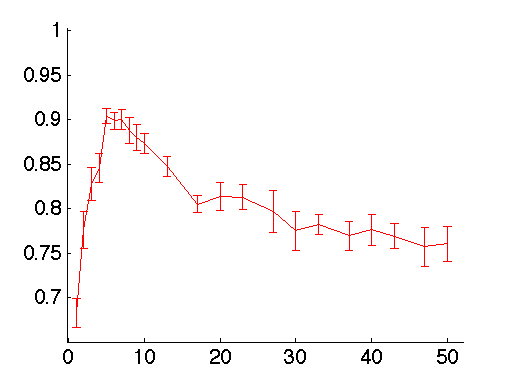
\includegraphics[width=.5\textwidth]{../images/nb_acc_vs_dim_pca_sr.png}}
\subfloat[SVM]{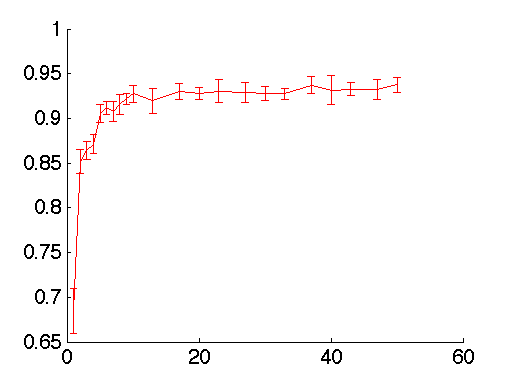
\includegraphics[width=.5\textwidth]{../images/svm_acc_vs_dim_pca_sr.png}}
\caption{Accuracy vs. dim. PCA Projection}
\label{fig:pca_acc_vs_proj_dim}
\end{figure}

In analysis, here, mention something about how with svm model complexity scales with number of training examples, not dimensionality of feature space. Also, point out that it makes sense to use linear kernel, rather than rbf, because of COD. 

\begin{figure}[h!]
\centering
\subfloat[Reduced Data Sparsity]{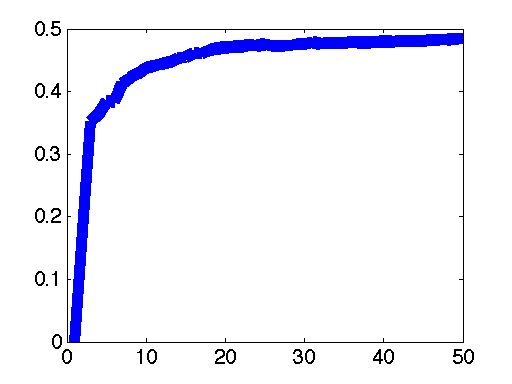
\includegraphics[width=.5\textwidth]{../images/PCAsparsityDensity.png}}
\subfloat[Cumulative Covariance]{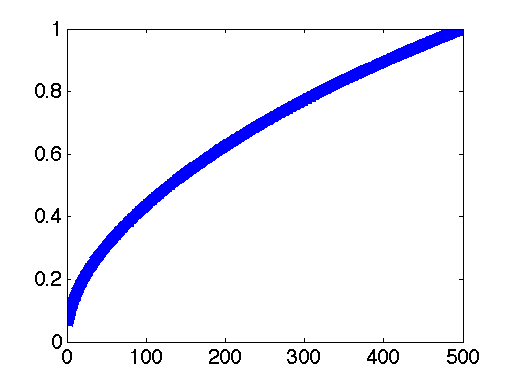
\includegraphics[width=.5\textwidth]{../images/pca_cumsum.png}}
\caption{Characteristics of PCA-reduced data}
\label{fig:PCA_RED}
\end{figure}

\begin{center}
\begin{figure}[h!]
\centering
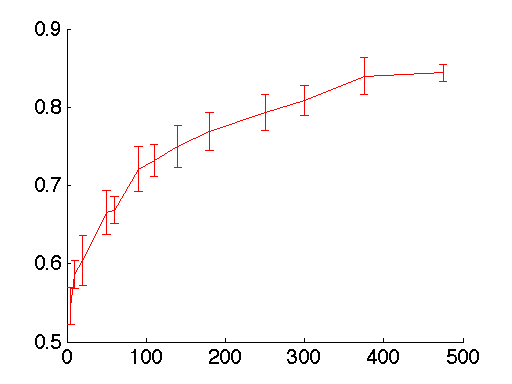
\includegraphics[width=.5\textwidth]{../images/accuracy_vs_dim_randproj.png}
\caption{Naive Bayes Acc. vs. num dim Rand. Projection}
\label{fig:nb_rand_proj}
\end{figure}
\end{center}

%also include naive bayes small pca vs. naive bayes pca. If it was just an issue of underfit gaussians, nonsmall would do better for bigger training sets, but it doesn't. 

\begin{center}
\begin{figure}[h!]
\centering
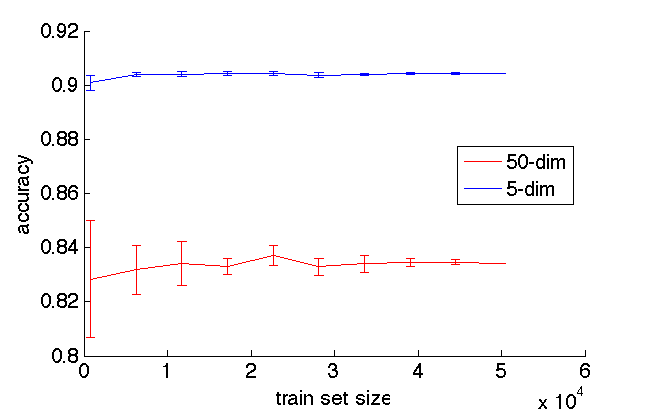
\includegraphics[width=.5\textwidth]{../images/nb_5_vs_50.png}
\caption{Naive Bayes Accuracy vs. Train set size for 5 and 50 PCA dims.}
\label{fig:5_vs_50_pca}
\end{figure}
\end{center}


\begin{figure}[h!]
\centering
\subfloat[L1 regularization]{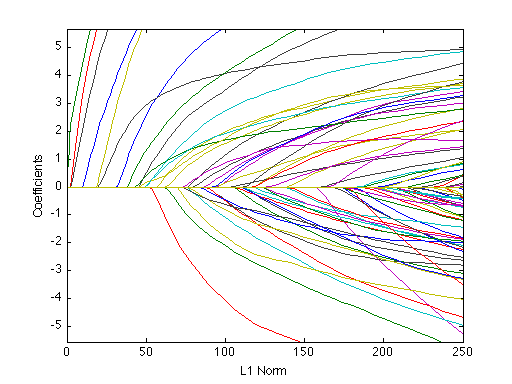
\includegraphics[width=.5\textwidth]{../images/lassoCoeffCurve.png}}
\subfloat[L2 regularization]{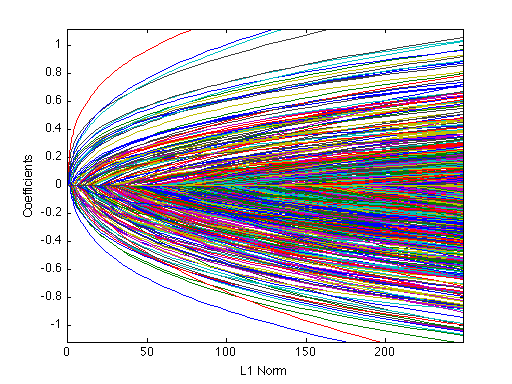
\includegraphics[width=.5\textwidth]{../images/ridgeCoeffCurve.png}}
\caption{Coefficient Paths for Regularized Logistic Regression}
\label{fig:Coeff_paths}
\end{figure}

Citing...
\cite{ratinov2009design}

\bibliographystyle{plain}
\bibliography{citations}

\end{document}

